\documentclass[../main.tex]{subfiles}

\begin{document}

The process executor receives at input a process context, which consists of:
\begin{itemize}
    \item \textbf{command:} command to be executed by the process executor, e.g. \textit{git init --bare}

    \item \textbf{working directory:} the directory where should be the command executed

    \item \textbf{extra environment variables:} additional environment variables just for the process

    \item \textbf{STDOUT consumer:} consumer of the standard output of the executed process

    \item \textbf{STDERR consumer:} consumer of the standard error output of the executed process
\end{itemize}

Afterwards, it starts executing the provided command and redirecting stdout and stderr into its corresponding consumers. Once the command is finished, the process executor returns its exit code. The design of the process executor is visualized in the Figure \ref{fig:process-executor}.

\begin{figure}
  \begin{center}
    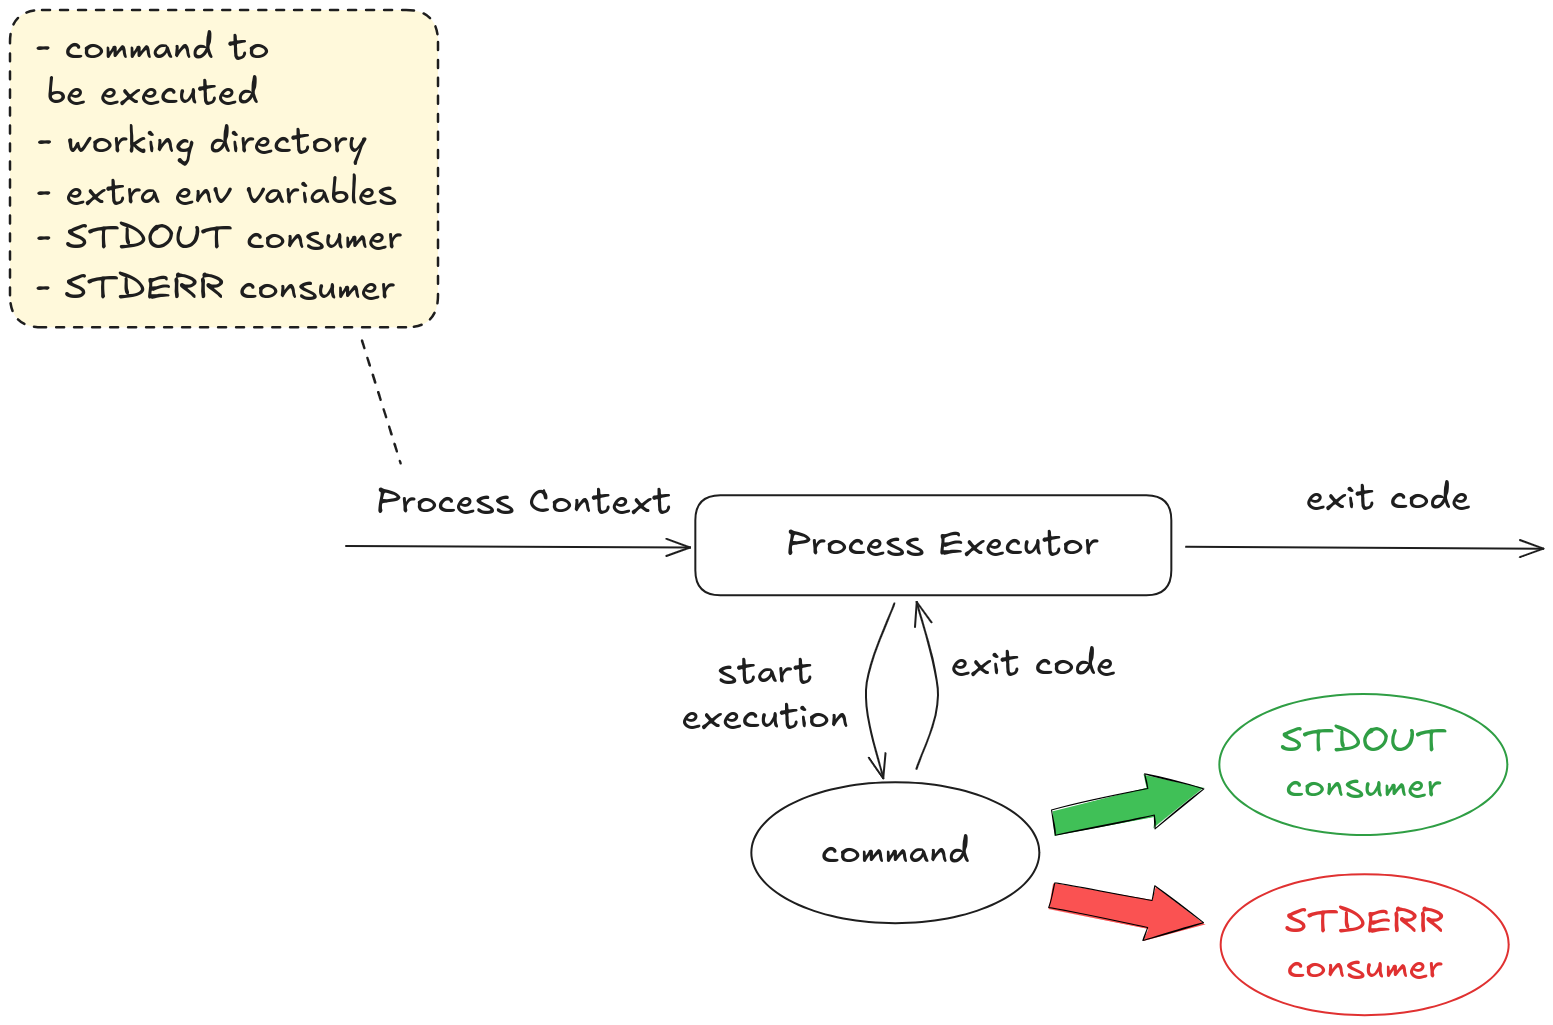
\includegraphics[width=\textwidth]{images/process-executor.png}
  \end{center}
  \caption{High-level overview of process executor}
  \label{fig:process-executor}
\end{figure}

\end{document}
